\section{CompCert's Correctness}
\label{sec:correctness}

Our picture of CompCert from \secref{terminology} was:

\begin{center}
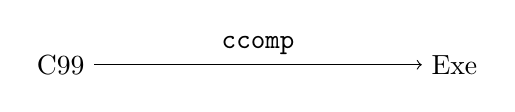
\begin{tikzpicture}
  \node (0) {C99};
  \node (1) [right of=0,xshift=4cm]{Exe};
  \draw[->] (0) -- node[above]{{\tt ccomp}} (1);
\end{tikzpicture}
\end{center}

but CompCert does not guarantee that every executable it generates simulates the original C99 program.
For one, the C99 standard does not include a formal semantics.
It leaves some behaviors undefined, like the order that function arguments are evaluated.
Also the executable does not have formal semantics modeled in Coq, and all CompCert's guarantees are Coq theorems.
The true picture is:
\begin{center}
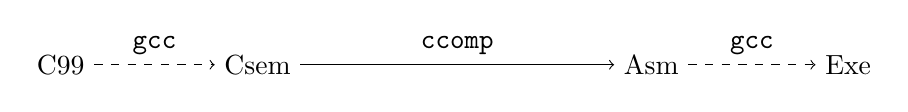
\begin{tikzpicture}
  \node (0) {Csem};
  \node (1) [right of=0,xshift=4cm]{Asm};
  \node (2) [left of=0,xshift=-1.5cm] {C99};
  \node (3) [right of=1,xshift=1.5cm] {Exe};
  \draw[->,dashed] (2) -- node[above]{{\tt gcc}} (0);
  \draw[->] (0) -- node[above]{{\tt ccomp}} (1);
  \draw[->,dashed] (1) -- node[above]{{\tt gcc}} (3);
\end{tikzpicture}
\end{center}
Where \href{https://github.com/AbsInt/CompCert/blob/master/cfrontend/Csem.v}{Csem} is CompCert's semantics for C99 (after preprocessing)
 and \href{https://github.com/AbsInt/CompCert/blob/master/ia32/Asm.v}{Asm} is CompCert's model of assembly language.\footnote{Either PowerPC, ARM, or \intel}
The dashed arrows are not verified, with the exception of the parsing stage (see \secref{menhir}, below).
Moreover, the solid arrow from Csem to Asm is divided into many smaller arrows; one for each pass described in \secref{passes}.

\subsection{Caveats}
Compiler correctness is built from small proofs of each pass, but before we can state the proper theorem we must address two pitfalls.

First, {\bf non-determinism} can raise issues when it is present in either the target or source languages.
Non-determinism in the \emph{target} language makes forward simulation proofs less effective.
Showing that all source behaviors are matched by a target behavior is good, but there could be additional target behaviors that shows up at runtime.
(Non-determinism means there's a choice both at proof-time and run-time.)
CompCert solves this by additionally proving that all target languages are deterministic.

Non-determinism in the \emph{source} language conversely makes backward simulations less appealing, because the proof only needs to work for one of the possible source transitions.
Unfortunately the non-determinism in C99 is unavoidable (at least until Airbus starts using the 2020 CompCert C standard).
CompCert's position is to \emph{choose one} of the source program's potential behaviors.
This is documented the source code as CompCert's \href{https://github.com/AbsInt/CompCert/blob/master/cfrontend/Cstrategy.v}{reduction strategy}, as opposed to the \href{https://github.com/AbsInt/CompCert/blob/master/cfrontend/Csem.v}{valid semantics} listed.

Second, {\bf diverging} source programs present a difficulty.
Should a verified compiler guarantee that all diverging source programs become diverging assembly programs?
It is impossible to tell whether a source program will diverge or not, so preserving divergence would either require the compiler to be extremely faithful to the source program's semantics (read: optimize less) or force it to conservatively fail on more programs (because a verified compiler may reject as many programs as it likes).
Neither solution is ideal; consider the dead-code optimization:

\hbox{
\begin{lstlisting}
int y = 4 / 0;
return 4;
\end{lstlisting}\becomes\begin{lstlisting}
noop;
return 4;
\end{lstlisting}
}

The source program diverges, but the target halts.
Nonetheless, dead-code elimination is a pragmatic optimization.

CompCert takes a ``garbage in, garbage out'' stance.
If the source program is unsafe or demonstrates undefined behavior, the correctness theorem does not hold.
The only guarantees are for converging source programs.


\subsection{CompCert's Correctness}

Compiler correctness is stated as the composition of smaller theorems for each pass.
\begin{itemize}
\item
  Each pass between C CompCert C (the determinisitic semantics) and Asm is proved using a forward simulation.
  Some of these simulations are measured, but others are in one-to-one correspondence.
\item
  Forward simulations from RTL to Asm, from Cminor to Asm, and from Cstrategy to Asm are derived as the composition of pass simulations.
\item
  Backward simulations for each of these 3 pairs of languages are derived from the forward simulations.
\item
  The final theorem: Csem is in backwards simulation with the CompCert C strategy, and thereby with Asm.
\end{itemize}
We can paraphrase this result as ``every observable Asm behavior is an observable target behavior''.

The Coq \href{https://github.com/AbsInt/CompCert/blob/master/driver/Compiler.v#L367}{theorem} is:
\begin{lstlisting}[style=Coq]
Theorem transf_c_program_correct:
  forall p tp,
  transf_c_program p = OK tp ->
  backward_simulation (Csem.semantics p) (Asm.semantics tp).
\end{lstlisting}


\subsection{Missing Theorems}

CompCert does \emph{not} prove some desirable properties:
\begin{itemize}
\item Semantics-preserving preprocessing
\item Safe assembling, safe linking
\item Whether compilation halts (the OCaml heuristics or unverified portions might loop forever)
\item Whether the executable is free of segfaults or null pointer exceptions
\item Time / space efficiency of the compiler
\item Time / space efficiency of the generated code
\item Anything about threaded programs
\end{itemize}

Some of these are failures of CompCert, others are failures of C.
They are all opportunities for improvement.


%% \subsection{Stuttering Simulation}
%% Alternative, by Namjoshi and Zuck~\cite{nz-witnessing}.
%% Change your heuristic functions to produce witness relations.
%% The witnesses relate source and target states with a stuttering simulation.

%% A stuttering simulation
%% - relates initial states
%% - if source takes a step, for all targets related to the source we have:
%% -- target steps to a related target
%% -- target steps to a target related to the INITIAL source
%% -- target steps to a target, and INITIAL target related to the source
%% In the latter two cases, we decrease along a well-founded measure.

%% Simulations compose without rank; I'm not sure how they compose with rank.
%% Unless there's a ``sync point'' at the end of one transformation where we can ``reset'' the measure.

%% The point of stuttering simulations is that they imply implementation.
%% Target code implements source if every terminating computation of target can be matched to a terminating computation of source using a given relation R.
%% R is the stuttering simulation.
%% Implementation is supposed to be a good notion of compiler correctness.

%% The authors show how stuttering simulation could prove hoisting and loop reordering.
%%  i.e. moving statements out-of-loop
%%       and changing the for-loop domain
%% Does CompCert do these?


%% \subsection{Notes}

%% On paper, the proof would take hundreds of pages~\cite{refman}.

